\documentclass[10pt,letterpaper]{report}
\usepackage[utf8]{inputenc}
\usepackage{amsmath}
\usepackage{amsfonts}
\usepackage{amssymb}
\usepackage{graphicx}
\usepackage{subfig}
\author{Brandon Houghton}
\begin{document}


In this period we finished work on integrating new datasets into our framework. Pendulum data is able to be simulated quickly enough that calculating pendulum trajectories during training is viable, however for turbulence data our current approach uses a single large simulated result and subsamples from it. Simulated turbulence data represents a 2D field with roughly 275 by 360 samples over 1000 time steps. Training using this data will be achieved by selecting arbitrary squares of the vorticity field for 200 time steps for random start simulation time. 

In order to adapt this turbulence data, we need the gradient of the vorticity field, which is not in the simulated data, therefore we approximate the derivative via central-finite distance given by $ dt(F_{t+1} - F_{t-1}) $ illustrated in figure 1.

\begin{figure}
\begin{center}
	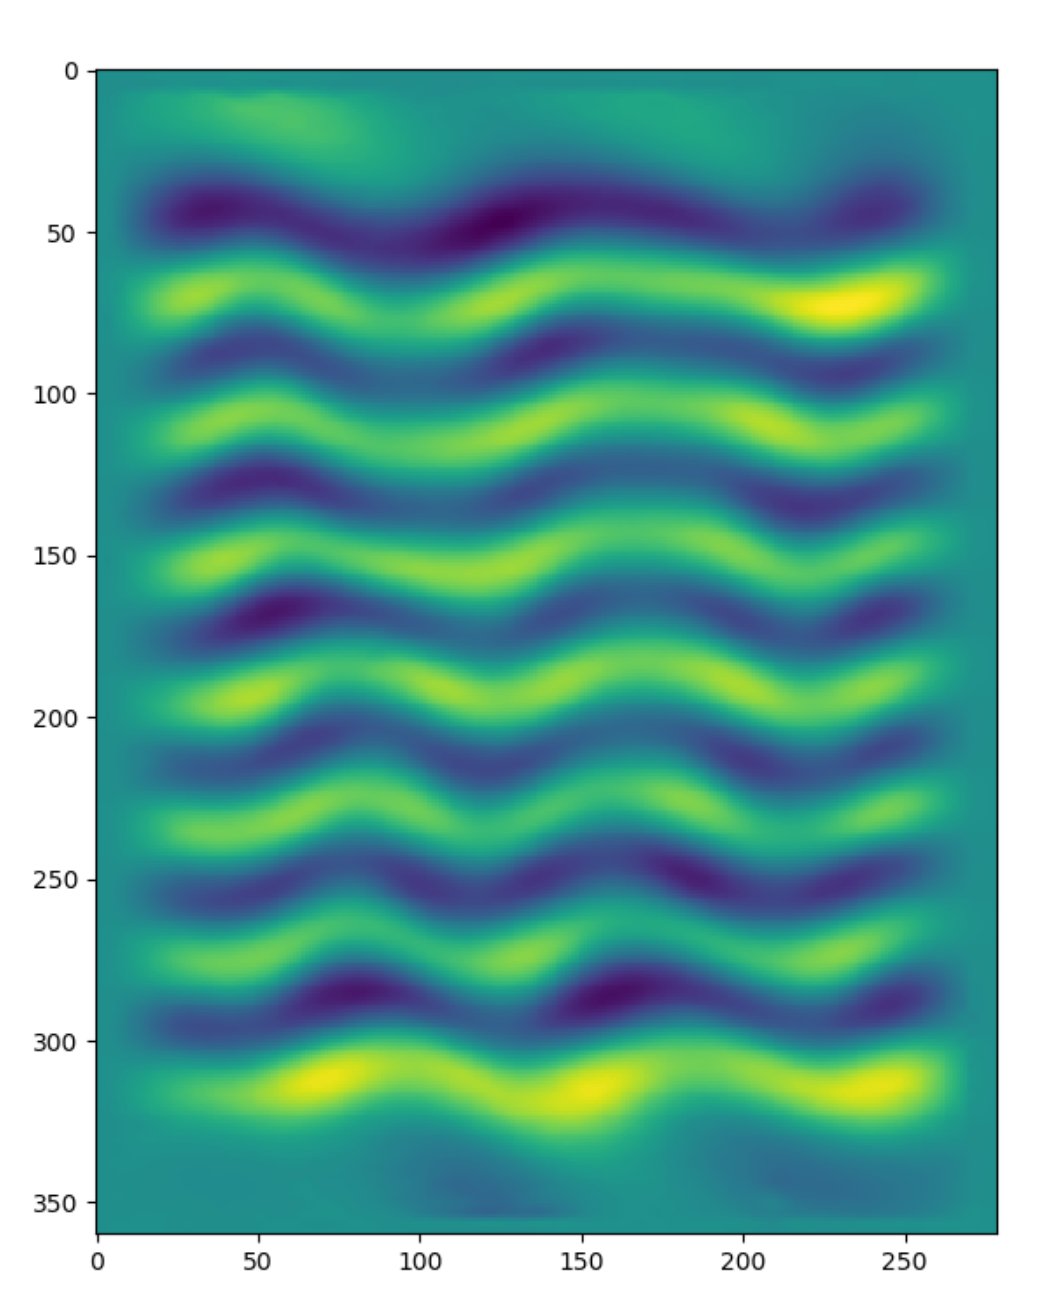
\includegraphics[width=0.49\textwidth]{vortex.png}
	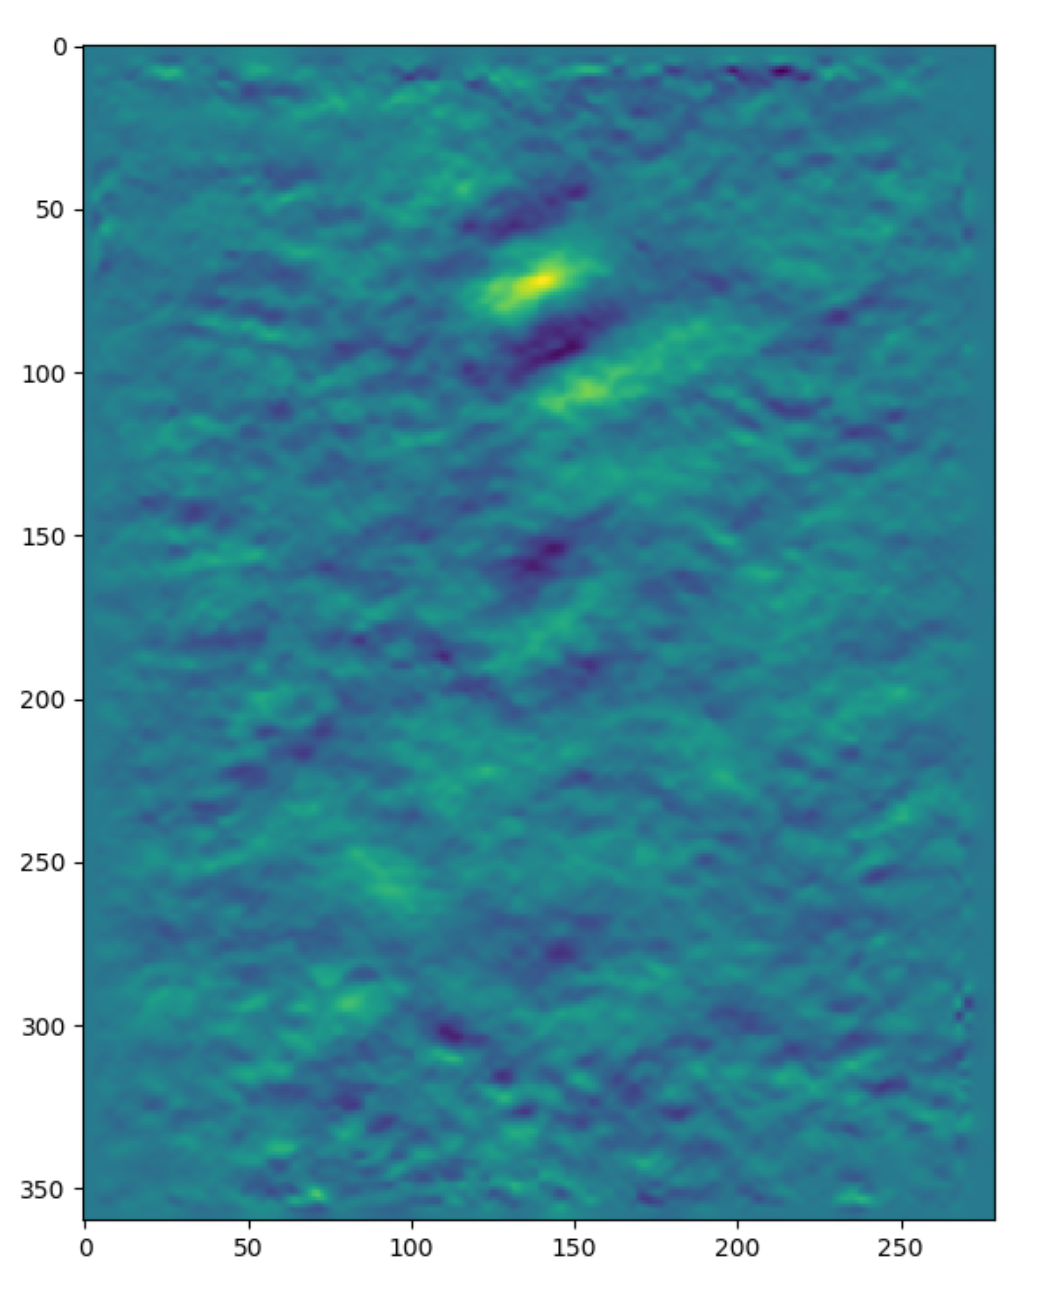
\includegraphics[width=0.49\textwidth]{vortex_der.png}
	\caption{\small (Left) Vorticity field $F$ at $t=1$. (Right)  Finite distance approximation of the time-derivative $\nabla_t F$ of vorticity field. }
\end{center}	
\end{figure}





\end{document}